\documentclass[11pt,a4paper]{article}

% ---------- packages ----------
\usepackage[margin=2.2cm,top=2.4cm,bottom=2.4cm]{geometry}
\usepackage[T1]{fontenc}
\usepackage{amsmath,amssymb}
\usepackage{helvet}
\renewcommand{\familydefault}{\sfdefault}
\usepackage{microtype}
\usepackage[table]{xcolor}
\usepackage{booktabs}
\usepackage{colortbl}
\usepackage{array}
\usepackage{tabularx}
\usepackage{caption}
\usepackage{float}
\usepackage{titlesec}
\usepackage{fancyhdr}
\usepackage{tcolorbox}
\tcbuselibrary{skins}
\usepackage{pgfplots}
\pgfplotsset{compat=1.18}
\usetikzlibrary{patterns}
\usepackage[hidelinks]{hyperref}

% ---------- NVIDIA palette ----------
\definecolor{nvgreen}{HTML}{76B900}
\definecolor{nvdark}{HTML}{1A1A1A}
\definecolor{nvgrey}{HTML}{4F4F4F}
\definecolor{nvlight}{HTML}{F2F2F2}
\definecolor{nvrule}{HTML}{D0D0D0}

% ---------- section style ----------
\titleformat{\section}
  {\sffamily\bfseries\large\color{nvgreen}}
  {\thesection}{0.6em}{}[\vspace{-0.4em}\textcolor{nvrule}{\rule{\linewidth}{0.6pt}}]
\titleformat{\subsection}
  {\sffamily\bfseries\normalsize\color{nvdark}}
  {\thesubsection}{0.5em}{}

% ---------- header / footer ----------
\pagestyle{fancy}
\fancyhf{}
\renewcommand{\headrulewidth}{0pt}
\renewcommand{\footrulewidth}{0pt}
\fancyhead[L]{\footnotesize\textcolor{nvgrey}{NVIDIA \textbar{} Isaac Lab Scaling Report}}
\fancyhead[R]{\footnotesize\textcolor{nvgrey}{Cable \& CablePlug}}
\fancyfoot[C]{\footnotesize\textcolor{nvgrey}{\thepage}}

% ---------- callout box ----------
\newtcolorbox{keybox}{
  colback=nvlight, colframe=nvgreen,
  boxrule=0pt, leftrule=4pt,
  arc=0pt, outer arc=0pt,
  left=10pt, right=10pt, top=8pt, bottom=8pt,
  enhanced, sharp corners,
}

% ---------- table style ----------
\renewcommand{\arraystretch}{1.15}

% ---------- pgfplots defaults ----------
\pgfplotsset{
  every axis/.append style={
    font=\small,
    axis line style={nvgrey},
    tick style={nvgrey},
    label style={nvdark},
    title style={nvdark},
    legend style={
      draw=nvrule,
      fill=white,
      font=\footnotesize,
    },
    grid style={nvrule, dashed},
  },
}

\begin{document}

% Suppress the fancyhdr header on the title page so it doesn't overlap
% the NVIDIA green title bar.
\thispagestyle{plain}
\fancypagestyle{plain}{%
  \fancyhf{}%
  \renewcommand{\headrulewidth}{0pt}%
  \fancyfoot[C]{\footnotesize\textcolor{nvgrey}{\thepage}}%
}

% =============== TITLE BLOCK ===============
\begin{tikzpicture}[remember picture, overlay]
  \fill[nvgreen]
    (current page.north west)
    rectangle ([yshift=-1.4cm]current page.north east);
  \node[anchor=west, text=white, font=\sffamily\bfseries\Large]
    at ([xshift=2.2cm, yshift=-0.7cm]current page.north west)
    {NVIDIA \textbar{} ISAAC LAB};
  \node[anchor=east, text=white, font=\sffamily]
    at ([xshift=-2.2cm, yshift=-0.7cm]current page.north east)
    {Internal technical report};
\end{tikzpicture}
\vspace*{1.0cm}

\noindent\textcolor{nvgrey}{\small \today \quad\textbar\quad Branch \texttt{max} \quad\textbar\quad Prepared by Maximilian Krause}
\vspace{0.3em}

\noindent{\sffamily\bfseries\Huge\color{nvdark} RL Training Throughput Scaling}\\[0.2em]
\noindent{\sffamily\Large\color{nvgrey} Isaac-..-v0 \& Isaac-...-v0}
\vspace{1.0em}

\noindent\textcolor{nvrule}{\rule{\linewidth}{0.6pt}}

% =============== EXECUTIVE SUMMARY ===============
\section*{\textcolor{nvgreen}{Executive summary}}
\addcontentsline{toc}{section}{Executive summary}

\begin{keybox}
\sffamily
\textbf{Cable env.} Total throughput scales with parallelism up to
\textbf{4{,}096 envs (23{,}917 steps/s)}, plateaus there, and \emph{regresses}
above 4{,}096 envs --- \textbf{6{,}144 envs is the first operating point where
adding more environments yields fewer samples per second}. Below 4{,}096 envs
the GPU still has headroom; above it, iteration time grows linearly with
\texttt{num\_envs} ($\approx 1.03$~ms/env) but throughput no longer climbs.

\medskip
\textbf{CablePlug env.} Scales \emph{poorly}: total throughput
\textbf{peaks at only $\sim$20 steps/s near 8--16 envs} and then declines.
Iteration time grows roughly $\mathcal{O}(N^{1.6\text{--}2})$ in
\texttt{num\_envs}; the simulator collection phase --- not the PPO update ---
is responsible for $>99\%$ of the cost.

\medskip
\textbf{Proxy vs.\ ADMM coupling (Cable env).} ADMM on the plain cable
scene is $\sim$10$\times$ slower per iter than proxy at 8 envs, growing to
$\sim$53$\times$ at 32 envs; peak throughput stays $\leq$33~sps regardless
of \texttt{num\_envs}. The ADMM scaling on the cable scene closely mirrors
the CablePlug scaling, suggesting the ADMM solver itself is the dominant
cost in CablePlug.
\end{keybox}

% =============== METHODOLOGY ===============
\section{Methodology}

Each data point is one training run launched with
\begin{quote}\ttfamily\small
./isaaclab.sh train --rl\_library rsl\_rl --task \textit{\textless TASK\textgreater}\\
\hphantom{./isaaclab.sh train }--num\_envs \textit{N} --max\_iterations 20 --headless
\end{quote}
on a single NVIDIA RTX A6000 (49~GiB VRAM) in headless mode. The PPO trainer
(RSL-RL) uses \texttt{num\_steps\_per\_env~=~24}; the simulator uses
\texttt{decimation~=~1}, \texttt{sim.dt~=~1/60\,s}. The first three
iterations of every run are dropped as warm-up; reported numbers are the
mean over the remaining iterations. ``Steps per second'' is the value
RSL-RL prints to stdout, i.e.
$\text{num\_envs}\times\text{num\_steps\_per\_env}/\text{collection\_time}$.

\medskip
The metrics reported per run are:
\begin{itemize}\setlength\itemsep{0pt}
  \item \textbf{Iteration time} (s) --- wall-clock per RL iteration.
  \item \textbf{Steps per second} --- environment steps produced per
    wall-clock second.
  \item \textbf{Startup time} (s) --- time before the first training
    iteration starts producing samples.
  \item \textbf{Peak GPU memory} (MiB) --- training memory delta over
    the system baseline.
\end{itemize}

% =============== CABLE ENV ===============
\section{Isaac-Lift-Cable-Franka-v0}

\subsection{Scaling table}

\begin{table}[H]
\centering
\caption*{\sffamily\small\color{nvgrey}Cable env training throughput vs.\ number of parallel environments.}
\begin{tabular}{r r r r}
\toprule
\textbf{num\_envs} & \textbf{Iter time (s)} & \textbf{Steps / s} & \textbf{Steps / s / env}\\
\midrule
8     & 0.57 &    339 & 42.4 \\
16    & 0.60 &    643 & 40.2 \\
32    & 0.67 &  1{,}162 & 36.3 \\
64    & 0.69 &  2{,}232 & 34.9 \\
128   & 0.73 &  4{,}199 & 32.8 \\
256   & 0.81 &  7{,}580 & 29.6 \\
384   & 0.94 &  9{,}839 & 25.6 \\
512   & 1.03 & 11{,}939 & 23.3 \\
1{,}024  & 1.39 & 17{,}750 & 17.3 \\
2{,}048  & 2.23 & 22{,}008 & 10.8 \\
3{,}072  & 3.24 & 22{,}755 &  7.4 \\
\rowcolor{nvlight}\textbf{4{,}096}  & \textbf{4.11} & \textbf{23{,}917} & \textbf{5.8} \\
6{,}144  & 6.33 & 23{,}313 &  3.8 \\
8{,}192  & 8.54 & 23{,}052 &  2.8 \\
\bottomrule
\end{tabular}
\end{table}

\subsection{Throughput vs.\ number of envs}

\begin{figure}[H]
\centering
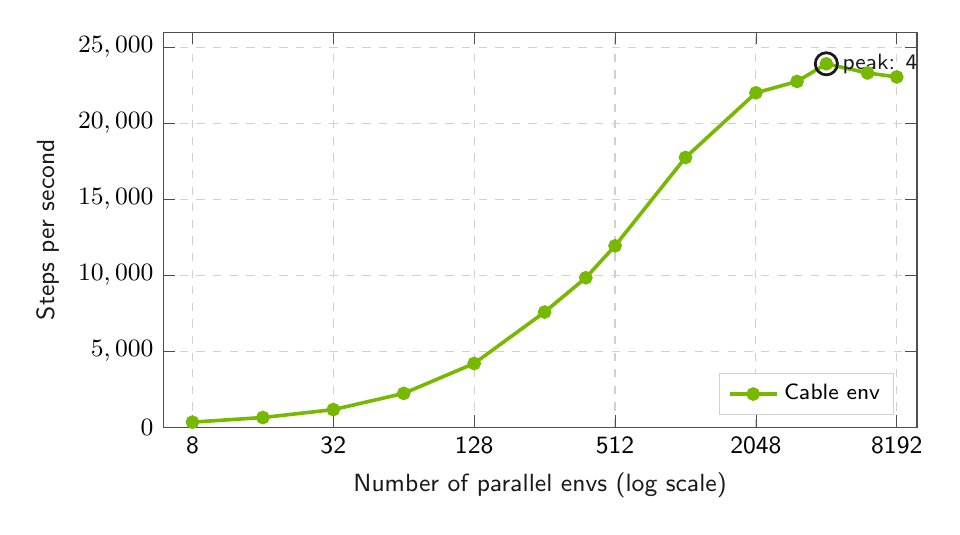
\begin{tikzpicture}
\begin{axis}[
  width=0.92\linewidth, height=6.6cm,
  xlabel={Number of parallel envs (log scale)},
  ylabel={Steps per second},
  xmode=log, log basis x=2,
  ymin=0, ymax=26000,
  xmin=6, xmax=10000,
  grid=both,
  legend pos=south east,
  scaled y ticks=false, y tick label style={/pgf/number format/.cd, fixed, 1000 sep={,}},
  xtick={8,32,128,512,2048,8192},
  xticklabels={8,32,128,512,2048,8192},
]
\addplot[
  color=nvgreen, line width=1.3pt,
  mark=*, mark options={fill=nvgreen, draw=nvgreen, scale=0.9},
] coordinates {
  (8,339) (16,643) (32,1162) (64,2232) (128,4199)
  (256,7580) (384,9839) (512,11939) (1024,17750)
  (2048,22008) (3072,22755) (4096,23917)
  (6144,23313) (8192,23052)
};
\addlegendentry{Cable env}

% peak marker
\addplot[only marks, mark=o, mark size=4pt, mark options={draw=nvdark, line width=1pt}]
  coordinates {(4096,23917)};
\node[anchor=west, font=\footnotesize\sffamily, text=nvdark]
  at (axis cs:4096,23917) {\;peak: 4{,}096 envs, 23{,}917 sps};
\end{axis}
\end{tikzpicture}
\caption*{\sffamily\small\color{nvgrey}Total throughput rises monotonically up to 4{,}096 envs, plateaus, then declines.}
\end{figure}

\subsection{Iteration time vs.\ number of envs}

\begin{figure}[H]
\centering
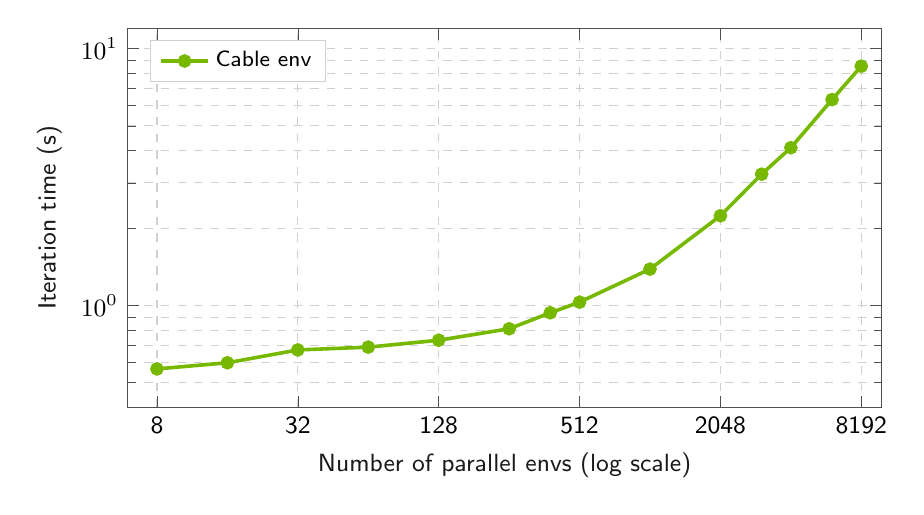
\begin{tikzpicture}
\begin{axis}[
  width=0.92\linewidth, height=6.4cm,
  xlabel={Number of parallel envs (log scale)},
  ylabel={Iteration time (s)},
  xmode=log, log basis x=2,
  ymode=log, log basis y=10,
  ymin=0.4, ymax=12,
  xmin=6, xmax=10000,
  grid=both,
  legend pos=north west,
  xtick={8,32,128,512,2048,8192},
  xticklabels={8,32,128,512,2048,8192},
]
\addplot[
  color=nvgreen, line width=1.3pt,
  mark=*, mark options={fill=nvgreen, draw=nvgreen, scale=0.9},
] coordinates {
  (8,0.566) (16,0.598) (32,0.671) (64,0.688) (128,0.732)
  (256,0.811) (384,0.936) (512,1.030) (1024,1.385)
  (2048,2.234) (3072,3.243) (4096,4.112)
  (6144,6.329) (8192,8.540)
};
\addlegendentry{Cable env}
\end{axis}
\end{tikzpicture}
\caption*{\sffamily\small\color{nvgrey}Iter time is nearly flat below 512 envs (kernel-launch dominated), then grows linearly above $\sim$2{,}048 envs ($\approx$1.03~ms/env) --- the GPU-saturation signature.}
\end{figure}

\subsection{When does adding more envs become a bad idea?}

\begin{itemize}\setlength\itemsep{2pt}
  \item \textbf{8 $\rightarrow$ 2{,}048 envs} --- strong scaling. Every
    doubling of \texttt{num\_envs} yields $\geq$24\% more throughput.
  \item \textbf{2{,}048 $\rightarrow$ 4{,}096 envs} --- diminishing returns.
    Each +1{,}024 envs adds only +3--5\% throughput.
  \item \textbf{4{,}096 envs} --- \emph{throughput peak} (23{,}917 sps).
  \item \textbf{$\geq$6{,}144 envs} --- net negative. Throughput is lower
    than at 4{,}096, iter time is longer, per-env efficiency is worse.
    Do not operate here.
\end{itemize}

% =============== PROXY vs ADMM ===============
\section{Proxy vs.\ ADMM coupling on the Cable env}

The Cable env above uses \textbf{proxy} coupling
(\texttt{CoupledProxySolverCfg}): the articulated robots are simulated in MJWarp while
cables are in VBD; the gripper fingers are exposed as virtual
proxies so VBD detects them as contacts on the cable. The cable plug env, by
contrast, uses \textbf{ADMM} coupling (\texttt{CoupledAdmmSolverCfg}), which
solves coupled mujoco-vbd constraints via an iterative
alternating-direction scheme. ADMM is more rigorous but more expensive per
step.

To compare the two on the same scene, the Cable env was re-instantiated
with the ADMM solver and the ADMM recipe used by the cable plug env
(iterations = 5, $\rho = 30$, $\gamma = 0.1$, baumgarte = 0.005, contact
distance = 0.003, VBD $\beta = 10^3$, \texttt{num\_substeps = 10}, contact
stiffness $k_e = 10^5$). Task registered as
\texttt{Isaac-Lift-Cable-ADMM-Franka-v0}.

\subsection{Side-by-side scaling}

\begin{table}[H]
\centering
\caption*{\sffamily\small\color{nvgrey}Cable env throughput with proxy vs.\ ADMM coupling.}
\begin{tabular}{r r r r r}
\toprule
& \multicolumn{2}{c}{\textbf{Proxy}} & \multicolumn{2}{c}{\textbf{ADMM}}\\
\cmidrule(lr){2-3}\cmidrule(lr){4-5}
\textbf{num\_envs} & \textbf{Iter (s)} & \textbf{Steps / s} & \textbf{Iter (s)} & \textbf{Steps / s}\\
\midrule
2    &  --- &     --- &  3.36 & 13.9 \\
4    &  --- &     --- &  4.01 & 23.6 \\
8    & 0.57 &     339 &  5.76 & 32.7 \\
16   & 0.60 &     643 & 11.82 & 32.3 \\
32   & 0.67 &  1{,}162 & 35.71 & 21.4 \\
\bottomrule
\end{tabular}
\end{table}

\subsection{Throughput vs.\ number of envs}

\begin{figure}[H]
\centering
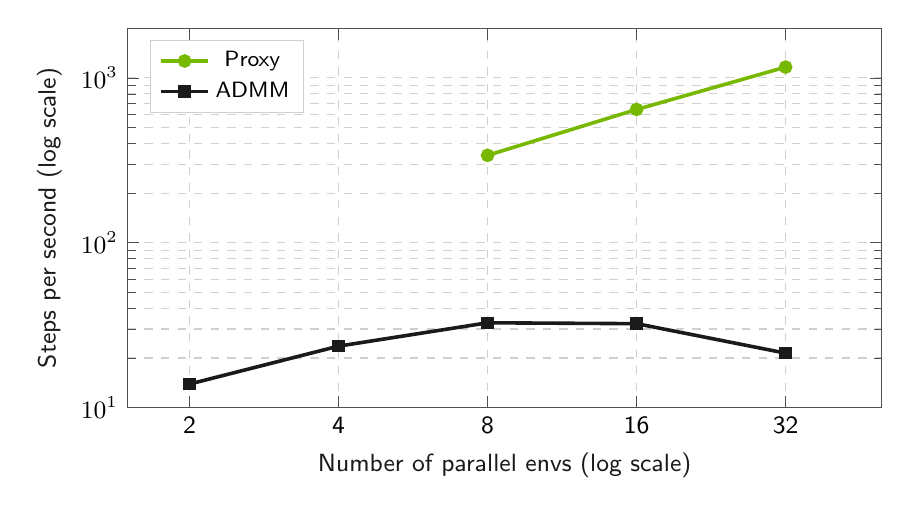
\begin{tikzpicture}
\begin{axis}[
  width=0.92\linewidth, height=6.4cm,
  xlabel={Number of parallel envs (log scale)},
  ylabel={Steps per second (log scale)},
  xmode=log, log basis x=2,
  ymode=log, log basis y=10,
  ymin=10, ymax=2000,
  xmin=1.5, xmax=50,
  grid=both,
  legend pos=north west,
  xtick={2,4,8,16,32},
  xticklabels={2,4,8,16,32},
]
\addplot[color=nvgreen, line width=1.3pt, mark=*, mark options={fill=nvgreen, scale=0.9}]
  coordinates {(8,339) (16,643) (32,1162)};
\addlegendentry{Proxy}
\addplot[color=nvdark, line width=1.3pt, mark=square*, mark options={fill=nvdark, scale=0.8}]
  coordinates {(2,13.9) (4,23.6) (8,32.7) (16,32.3) (32,21.4)};
\addlegendentry{ADMM}
\end{axis}
\end{tikzpicture}
\caption*{\sffamily\small\color{nvgrey}Proxy throughput grows linearly with \texttt{num\_envs}; ADMM throughput plateaus near 32~sps at 8--16 envs and then degrades. At 32 envs the proxy variant produces $\sim$54$\times$ more samples per second.}
\end{figure}

\subsection{Iteration time vs.\ number of envs}

\begin{figure}[H]
\centering
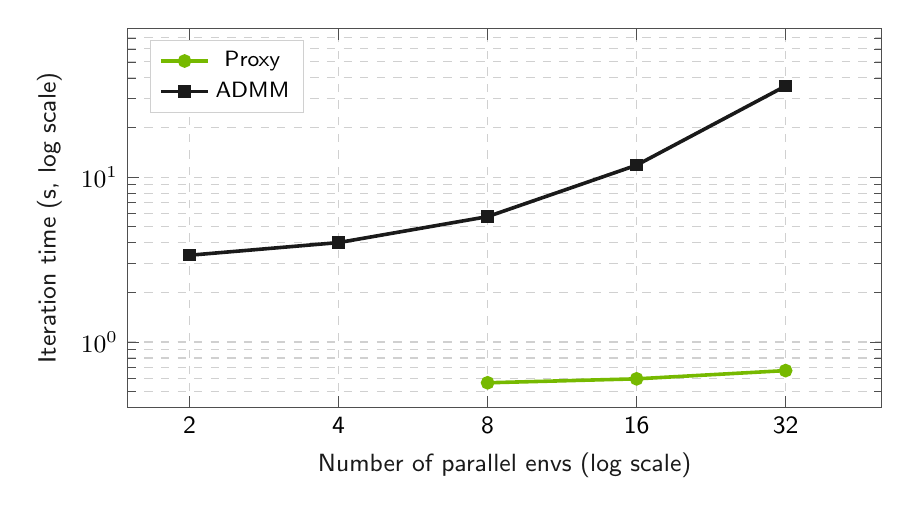
\begin{tikzpicture}
\begin{axis}[
  width=0.92\linewidth, height=6.4cm,
  xlabel={Number of parallel envs (log scale)},
  ylabel={Iteration time (s, log scale)},
  xmode=log, log basis x=2,
  ymode=log, log basis y=10,
  ymin=0.4, ymax=80,
  xmin=1.5, xmax=50,
  grid=both,
  legend pos=north west,
  xtick={2,4,8,16,32},
  xticklabels={2,4,8,16,32},
]
\addplot[color=nvgreen, line width=1.3pt, mark=*, mark options={fill=nvgreen, scale=0.9}]
  coordinates {(8,0.566) (16,0.598) (32,0.671)};
\addlegendentry{Proxy}
\addplot[color=nvdark, line width=1.3pt, mark=square*, mark options={fill=nvdark, scale=0.8}]
  coordinates {(2,3.36) (4,4.01) (8,5.76) (16,11.82) (32,35.71)};
\addlegendentry{ADMM}
\end{axis}
\end{tikzpicture}
\caption*{\sffamily\small\color{nvgrey}Proxy iter time is flat at $\sim$0.6~s across this range; ADMM iter time grows roughly linearly above 8 envs and is already 53$\times$ proxy at 32 envs.}
\end{figure}

\subsection{Interpretation}

\begin{itemize}\setlength\itemsep{2pt}
  \item \textbf{Per-iteration overhead.} At 8 envs, ADMM is $\sim$10$\times$
    slower than proxy (5.76~s vs.\ 0.57~s); at 32 envs the gap widens to
    $\sim$53$\times$ (35.71~s vs.\ 0.67~s). Proxy iter time barely moves
    with \texttt{num\_envs} in this range, while ADMM iter time scales
    super-linearly above 8 envs.
  \item \textbf{Throughput.} Proxy throughput rises linearly with envs in
    this range (339 $\rightarrow$ 1{,}162 sps for 8 $\rightarrow$ 32
    envs); ADMM peaks at $\sim$33 sps near 8--16 envs and \emph{drops} to
    21 sps at 32 envs.
  \item \textbf{Why use ADMM at all?} ADMM is required by the cable plug
    env because the plug couples back into the cable through rigid--soft
    attachments that proxy coupling cannot represent. For the plain cable
    env where the gripper is the only rigid contact, proxy coupling is the
    correct choice: same physical scene, $\geq$50$\times$ better throughput,
    no stability issues observed.
  \item \textbf{Implication for the cable plug env.} The super-linear
    cost growth observed earlier in the CablePlug env
    ($\mathcal{O}(N^{1.6\text{--}2})$) is consistent with ADMM's scaling
    on the plain cable scene, which suggests the ADMM solver itself ---
    not the plug geometry --- is the dominant source of cost in the cable
    plug benchmarks.
\end{itemize}

% =============== CABLE PLUG ENV ===============
\section{Isaac-Lift-CablePlug-Franka-v0}

\subsection{Scaling table}

\begin{table}[H]
\centering
\caption*{\sffamily\small\color{nvgrey}CablePlug env training throughput vs.\ number of parallel environments.}
\begin{tabular}{r r r r}
\toprule
\textbf{num\_envs} & \textbf{Iter time (s)} & \textbf{Steps / s} & \textbf{Steps / s / env}\\
\midrule
4     &   6.43 & 14.4 & 3.59 \\
\rowcolor{nvlight}\textbf{8} & \textbf{9.45} & \textbf{20.0} & \textbf{2.50} \\
16    &  20.10 & 18.9 & 1.18 \\
32    &  65.87 & 11.4 & 0.36 \\
64    & 288.88 &  5.1 & 0.08 \\
\bottomrule
\end{tabular}
\end{table}

\subsection{Throughput vs.\ number of envs}

\begin{figure}[H]
\centering
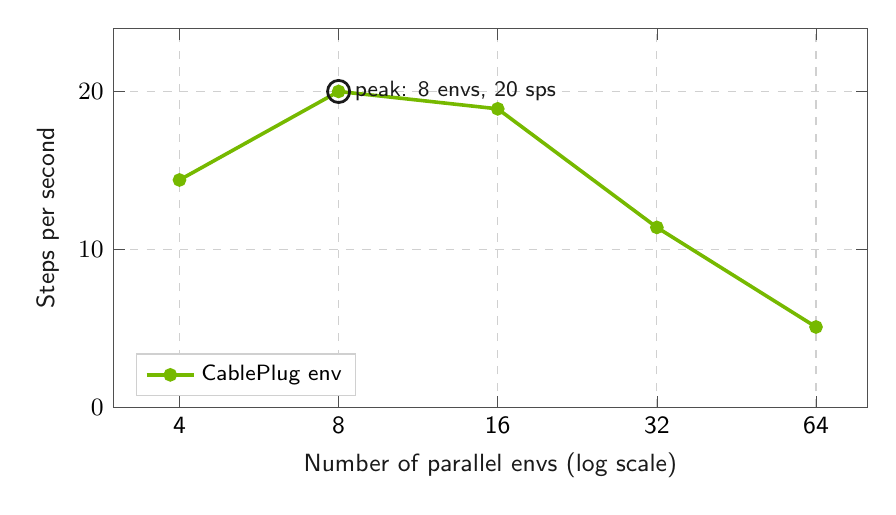
\begin{tikzpicture}
\begin{axis}[
  width=0.92\linewidth, height=6.4cm,
  xlabel={Number of parallel envs (log scale)},
  ylabel={Steps per second},
  xmode=log, log basis x=2,
  ymin=0, ymax=24,
  xmin=3, xmax=80,
  grid=both,
  legend pos=south west,
  xtick={4,8,16,32,64},
  xticklabels={4,8,16,32,64},
]
\addplot[
  color=nvgreen, line width=1.3pt,
  mark=*, mark options={fill=nvgreen, draw=nvgreen, scale=0.9},
] coordinates {
  (4,14.4) (8,20.0) (16,18.9) (32,11.4) (64,5.1)
};
\addlegendentry{CablePlug env}

\addplot[only marks, mark=o, mark size=4pt, mark options={draw=nvdark, line width=1pt}]
  coordinates {(8,20.0)};
\node[anchor=west, font=\footnotesize\sffamily, text=nvdark]
  at (axis cs:8,20.0) {\;peak: 8 envs, 20 sps};
\end{axis}
\end{tikzpicture}
\caption*{\sffamily\small\color{nvgrey}Throughput peaks near 8--16 envs and falls thereafter --- the opposite of healthy parallel scaling.}
\end{figure}

\subsection{Iteration time vs.\ number of envs}

\begin{figure}[H]
\centering
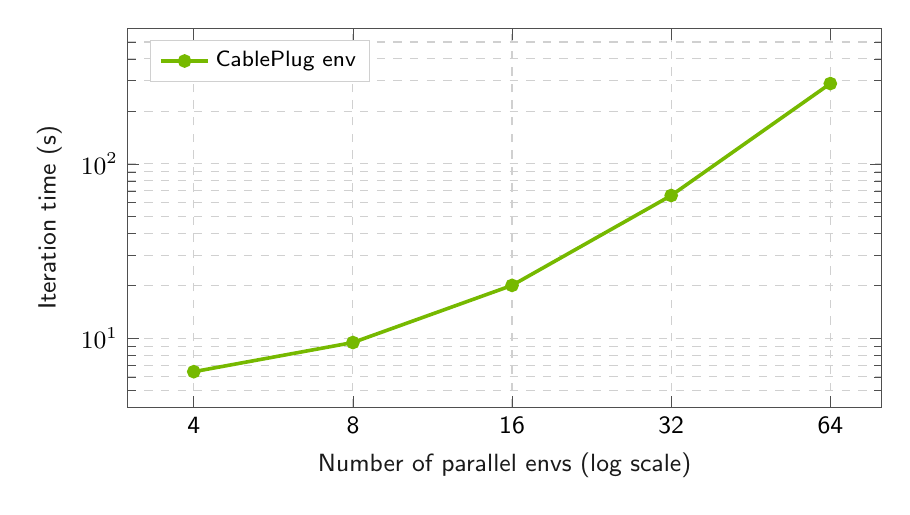
\begin{tikzpicture}
\begin{axis}[
  width=0.92\linewidth, height=6.4cm,
  xlabel={Number of parallel envs (log scale)},
  ylabel={Iteration time (s)},
  xmode=log, log basis x=2,
  ymode=log, log basis y=10,
  ymin=4, ymax=600,
  xmin=3, xmax=80,
  grid=both,
  legend pos=north west,
  xtick={4,8,16,32,64},
  xticklabels={4,8,16,32,64},
]
\addplot[
  color=nvgreen, line width=1.3pt,
  mark=*, mark options={fill=nvgreen, draw=nvgreen, scale=0.9},
] coordinates {
  (4,6.43) (8,9.45) (16,20.10) (32,65.87) (64,288.88)
};
\addlegendentry{CablePlug env}
\end{axis}
\end{tikzpicture}
\caption*{\sffamily\small\color{nvgrey}Iter time grows roughly $\mathcal{O}(N^{1.6\text{--}2})$ in \texttt{num\_envs}: doubling envs costs 3--4$\times$ more time per iteration.}
\end{figure}

\subsection{Implication}

For CablePlug, more parallel envs is actively harmful past $\sim$16. The
super-linear cost growth means the simulator does \emph{not} parallelize the
plug interactions efficiently; root-cause analysis of the collection phase
is needed before this task can use more envs productively.

% =============== HEAD TO HEAD ===============
\section{Head-to-head}

\begin{figure}[H]
\centering
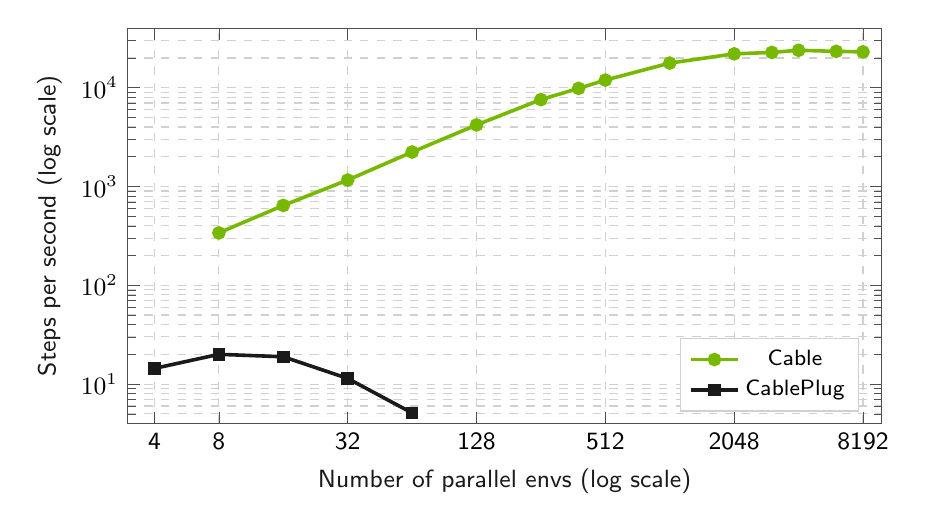
\begin{tikzpicture}
\begin{axis}[
  width=0.92\linewidth, height=6.6cm,
  xlabel={Number of parallel envs (log scale)},
  ylabel={Steps per second (log scale)},
  xmode=log, log basis x=2,
  ymode=log, log basis y=10,
  ymin=4, ymax=40000,
  xmin=3, xmax=10000,
  grid=both,
  legend pos=south east,
  xtick={4,8,32,128,512,2048,8192},
  xticklabels={4,8,32,128,512,2048,8192},
]
\addplot[color=nvgreen, line width=1.3pt, mark=*, mark options={fill=nvgreen, scale=0.9}]
  coordinates {
  (8,339) (16,643) (32,1162) (64,2232) (128,4199)
  (256,7580) (384,9839) (512,11939) (1024,17750)
  (2048,22008) (3072,22755) (4096,23917)
  (6144,23313) (8192,23052)};
\addlegendentry{Cable}
\addplot[color=nvdark, line width=1.3pt, mark=square*, mark options={fill=nvdark, scale=0.8}]
  coordinates {(4,14.4) (8,20.0) (16,18.9) (32,11.4) (64,5.1)};
\addlegendentry{CablePlug}
\end{axis}
\end{tikzpicture}
\caption*{\sffamily\small\color{nvgrey}Cable env achieves over 1{,}000$\times$ higher peak throughput than CablePlug env, and continues to scale well past 1{,}000 envs while CablePlug regresses past 16 envs.}
\end{figure}

% =============== STARTUP COST ===============
\section{Startup cost}

In addition to steady-state iteration time, every training run incurs a
one-time startup cost (Python imports, Isaac Sim app init, scene cloning,
USD stage build, RSL-RL setup) before the first training iteration produces
samples. At very large env counts this is no longer negligible.

\subsection{Startup time vs.\ number of envs}

\begin{table}[H]
\centering
\caption*{\sffamily\small\color{nvgrey}Startup time per run, by task and number of parallel envs.}
\begin{tabular}{r r r}
\toprule
\textbf{num\_envs} & \textbf{Cable startup (s)} & \textbf{CablePlug startup (s)}\\
\midrule
4       &    --- &  13.4 \\
8       &   11.3 &  13.3 \\
16      &   11.3 &  13.6 \\
32      &   11.8 &  14.9 \\
64      &   12.4 &  15.3 \\
128     &   13.7 & --- \\
256     &   16.6 & --- \\
384     &   19.3 & --- \\
512     &   22.2 & --- \\
1{,}024 &   32.2 & --- \\
2{,}048 &   53.7 & --- \\
3{,}072 &   75.1 & --- \\
4{,}096 &   96.2 & --- \\
6{,}144 &  142.2 & --- \\
8{,}192 &  188.6 & --- \\
\bottomrule
\end{tabular}
\end{table}

\begin{figure}[H]
\centering
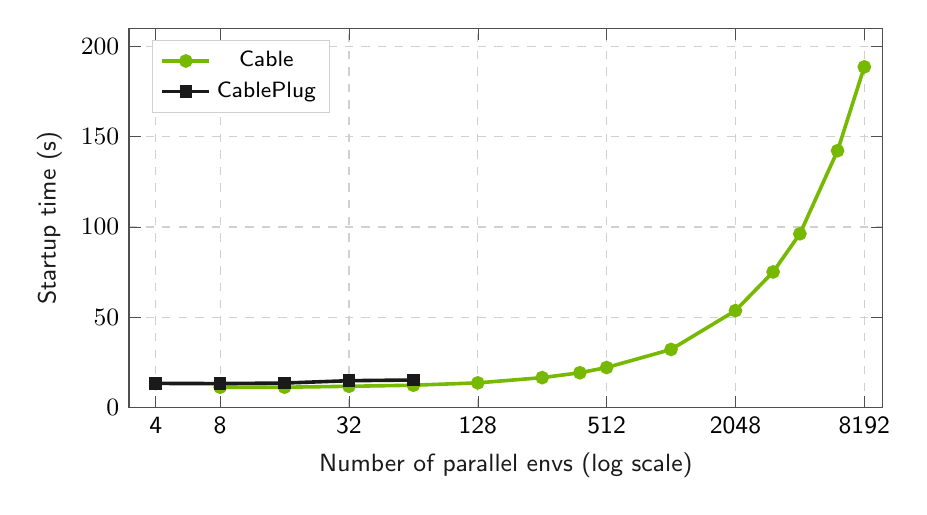
\begin{tikzpicture}
\begin{axis}[
  width=0.92\linewidth, height=6.4cm,
  xlabel={Number of parallel envs (log scale)},
  ylabel={Startup time (s)},
  xmode=log, log basis x=2,
  ymin=0, ymax=210,
  xmin=3, xmax=10000,
  grid=both,
  legend pos=north west,
  xtick={4,8,32,128,512,2048,8192},
  xticklabels={4,8,32,128,512,2048,8192},
]
\addplot[color=nvgreen, line width=1.3pt, mark=*, mark options={fill=nvgreen, scale=0.9}]
  coordinates {
  (8,11.3) (16,11.3) (32,11.8) (64,12.4) (128,13.7)
  (256,16.6) (384,19.3) (512,22.2) (1024,32.2)
  (2048,53.7) (3072,75.1) (4096,96.2) (6144,142.2) (8192,188.6)};
\addlegendentry{Cable}
\addplot[color=nvdark, line width=1.3pt, mark=square*, mark options={fill=nvdark, scale=0.8}]
  coordinates {(4,13.4) (8,13.3) (16,13.6) (32,14.9) (64,15.3)};
\addlegendentry{CablePlug}
\end{axis}
\end{tikzpicture}
\caption*{\sffamily\small\color{nvgrey}Cable env startup grows roughly linearly with \texttt{num\_envs} above $\sim$512 envs ($\approx$22~ms per added env). CablePlug startup is essentially flat (12--15~s) regardless of size --- the cable plug's expense is at simulation time, not at scene-clone time.}
\end{figure}

\subsection{Implication}

For long training runs (many thousands of iterations) the startup cost is
negligible. For shorter experiments at very large env counts it dominates:
\begin{itemize}\setlength\itemsep{2pt}
  \item Cable @ 8{,}192 envs: startup is 188.6~s --- more time than the
    first 22 training iterations combined.
  \item Cable @ 4{,}096 envs: startup of 96.2~s is roughly equal to the
    cost of 23 steady-state iterations.
  \item Cable @ 1{,}024 envs: startup of 32.2~s is roughly equal to 23
    iterations.
  \item Cable @ $\leq$256 envs: startup is essentially fixed at 11--17~s.
\end{itemize}

A useful rule of thumb on this branch and GPU: startup amortizes after
roughly 20--25 steady-state iterations, regardless of \texttt{num\_envs}.
Below that, smaller env counts have lower total wall-clock cost.

% =============== GPU MEMORY ===============
\section{GPU memory usage}

Peak GPU memory consumed by training, measured by polling
\texttt{nvidia-smi --query-gpu=memory.used} at 0.5~s intervals during a
short run (\texttt{--max\_iterations~2}) and subtracting the
pre-launch system baseline. The benchmark GPU is an NVIDIA RTX A6000 with
\textbf{49{,}140~MiB (48~GiB)} of VRAM.

\subsection{Memory vs.\ number of envs}

\begin{table}[H]
\centering
\caption*{\sffamily\small\color{nvgrey}Peak training GPU memory by task and number of parallel envs.}
\begin{tabular}{r r r}
\toprule
\textbf{num\_envs} & \textbf{Cable peak (GiB)} & \textbf{CablePlug peak (GiB)}\\
\midrule
2       &    --- & 0.70 \\
4       &    --- & 0.75 \\
8       &   0.49 & 0.80 \\
16      &   0.49 & 0.89 \\
32      &   0.49 & 2.18 \\
64      &   0.53 & --- \\
128     &   0.59 & --- \\
256     &   0.71 & --- \\
384     &   0.83 & --- \\
512     &   0.95 & --- \\
1{,}024 &   1.45 & --- \\
2{,}048 &   2.40 & --- \\
3{,}072 &   3.38 & --- \\
4{,}096 &   4.38 & --- \\
6{,}144 &   6.30 & --- \\
8{,}192 &   8.11 & --- \\
\bottomrule
\end{tabular}
\end{table}

\begin{figure}[H]
\centering
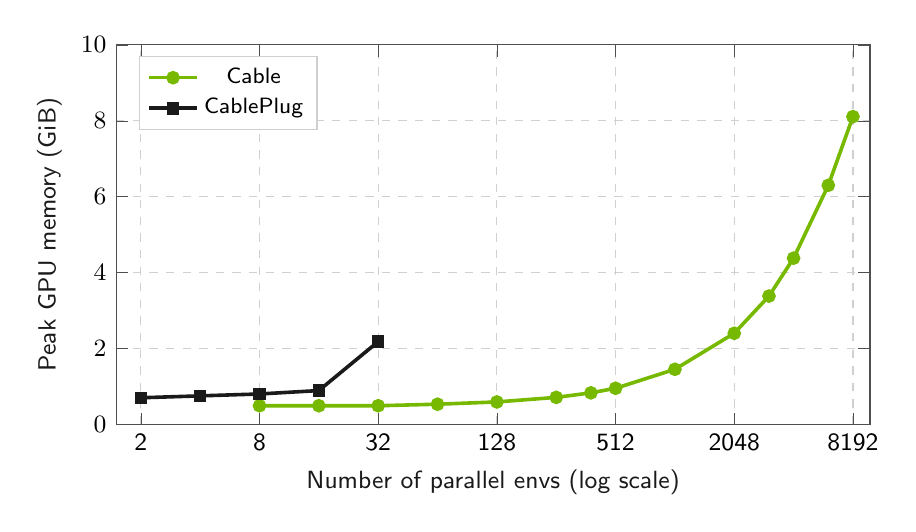
\begin{tikzpicture}
\begin{axis}[
  width=0.92\linewidth, height=6.4cm,
  xlabel={Number of parallel envs (log scale)},
  ylabel={Peak GPU memory (GiB)},
  xmode=log, log basis x=2,
  ymin=0, ymax=10,
  xmin=1.5, xmax=10000,
  grid=both,
  legend pos=north west,
  xtick={2,8,32,128,512,2048,8192},
  xticklabels={2,8,32,128,512,2048,8192},
]
\addplot[color=nvgreen, line width=1.3pt, mark=*, mark options={fill=nvgreen, scale=0.9}]
  coordinates {
  (8,0.49) (16,0.49) (32,0.49) (64,0.53) (128,0.59)
  (256,0.71) (384,0.83) (512,0.95) (1024,1.45)
  (2048,2.40) (3072,3.38) (4096,4.38) (6144,6.30) (8192,8.11)};
\addlegendentry{Cable}
\addplot[color=nvdark, line width=1.3pt, mark=square*, mark options={fill=nvdark, scale=0.8}]
  coordinates {(2,0.70) (4,0.75) (8,0.80) (16,0.89) (32,2.18)};
\addlegendentry{CablePlug}

% A6000 budget line
\addplot[dashed, color=nvgrey, line width=0.8pt, no marks]
  coordinates {(1.5,48) (10000,48)};
\end{axis}
\end{tikzpicture}
\caption*{\sffamily\small\color{nvgrey}Cable memory: fixed $\sim$0.5~GiB baseline for $\leq$32 envs, then grows linearly at $\approx$1~MiB per env. CablePlug memory: small ($\leq$1~GiB) below 32 envs, then a sharp step to 2.2~GiB at 32 envs. The 48~GiB A6000 budget is far above either trace.}
\end{figure}

\subsection{Implication}

\begin{itemize}\setlength\itemsep{2pt}
  \item Cable env memory is dominated by a fixed $\sim$0.5~GiB baseline
    (network weights, sim app, kit overhead) for env counts up to about 32,
    then grows linearly with \texttt{num\_envs} ($\approx$1~MiB per env)
    once cable storage dominates.
  \item At 8{,}192 envs Cable uses only 8.1~GiB --- about 17\% of A6000
    VRAM. \textbf{Memory is not the bottleneck} for Cable's throughput
    plateau at 4{,}096 envs; that plateau is computational.
  \item CablePlug shows a sharp memory jump from 0.89~GiB (16 envs) to
    2.18~GiB (32 envs). This is consistent with a per-env workspace that
    only allocates above a small threshold; the workspace is also the
    likely source of the super-linear iter-time growth in CablePlug.
\end{itemize}

% =============== TAKEAWAYS ===============
\section{Recommended operating points}

\begin{tabular}{l l l}
\toprule
\textbf{Task} & \textbf{Recommended num\_envs} & \textbf{Why}\\
\midrule
Cable     & \textbf{4{,}096} (max throughput) & Throughput peak. \\
Cable     & 2{,}048 (balanced)                & 92\% of peak at half the iter time. \\
Cable     & $\leq$1{,}024 (sample efficient)  & Per-env throughput $\geq$17 sps/env. \\
CablePlug & \textbf{8--16}                    & Throughput peak; above is regression. \\
\bottomrule
\end{tabular}

\vspace{0.5em}
\noindent\textcolor{nvgrey}{\footnotesize All raw per-run JSON and stdout logs are kept under \texttt{/tmp/cable\_scaling/results/}.}

\end{document}